\documentclass{standalone}
\usepackage{tikz}
\usetikzlibrary{positioning}

\begin{document}
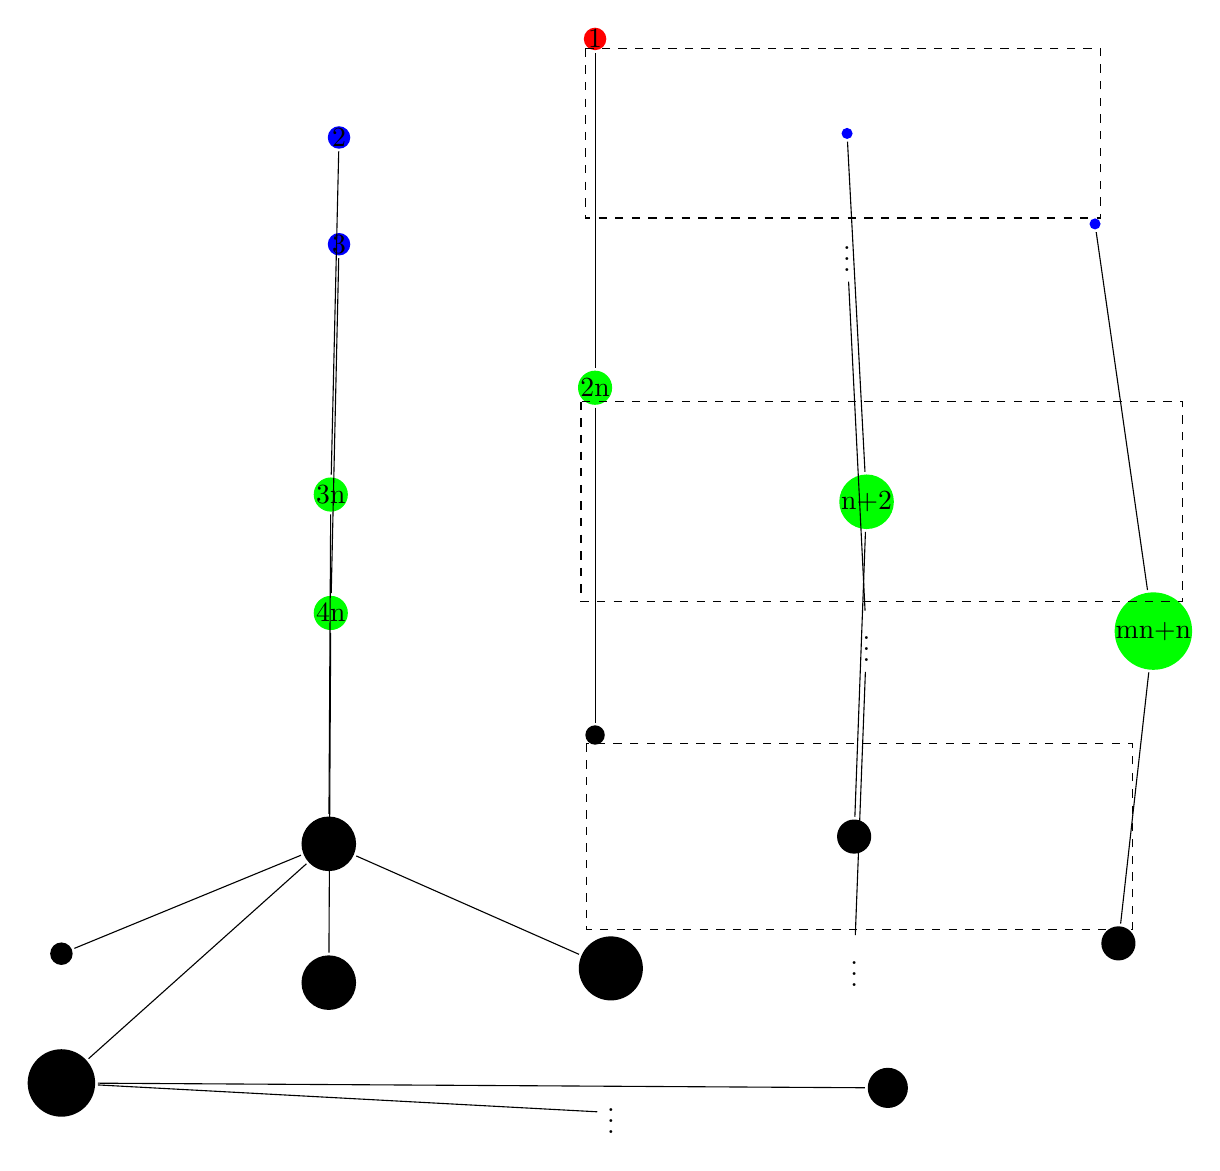
\begin{tikzpicture}[node distance=1cm and 3cm,
    dot/.style={circle,fill=#1,minimum size=4pt,inner sep=0pt,outer sep=1pt},
    dot/.default=black]

    % Define nodes for the top-level structure
    \node[dot=red] (top1) {1};
    \node[dot=blue,below left=of top1] (top2) {2};
    \node[dot=blue,below=of top2] (top3) {3};
    \node[dot=blue,below right=of top1] (top4) {};
    \node[below=of top4] (top5) {$\vdots$};
    \node[dot=blue,below right=of top4] (top6) {};

    % Create a dashed rectangle around the top nodes
    \draw[dashed] (top1.south west) rectangle (top6.north east);

    % Nodes for the second level
    \node[dot=green,below=4cm of top1] (mid1) {2n};
    \node[dot=green,below left=of mid1] (mid2) {3n};
    \node[dot=green,below=of mid2] (mid3) {4n};
    \node[dot=green,below right=of mid1] (mid4) {n+2};
    \node[below=of mid4] (mid5) {$\vdots$};
    \node[dot=green,below right=of mid4] (mid6) {mn+n};

    % Create a dashed rectangle around the mid nodes
    \draw[dashed] (mid1.south west) rectangle (mid6.north east);

    % Connect the top level to the second level
    \foreach \i in {1,...,6} {
        \draw (top\i) -- (mid\i);
    }

    % Nodes for the third level
    \node[dot=black,below=4cm of mid1] (low1) {n};
    \node[dot=black,below left=of low1] (low2) {n+1};
    \node[dot=black,below=of low2] (low3) {n+2};
    \node[dot=black,below right=of low1] (low4) {2n};
    \node[below=of low4] (low5) {$\vdots$};
    \node[dot=black,below right=of low4] (low6) {3n};

    % Create a dashed rectangle around the low nodes
    \draw[dashed] (low1.south west) rectangle (low6.north east);

    % Connect the second level to the third level
    \foreach \i in {1,...,6} {
        \draw (mid\i) -- (low\i);
    }

    % Additional node connections for the pattern
    \node[dot=black,below left=of low2] (low7) {2};
    \node[dot=black,below=of low7] (low8) {2n+1};
    \node[dot=black,below right=of low2] (low9) {mn-n};
    \node[below=of low9] (low10) {$\vdots$};
    \node[dot=black,below right=of low9] (low11) {mn};

    \draw (low2) -- (low7);
    \draw (low2) -- (low8);
    \draw (low2) -- (low9);
    \draw (low8) -- (low10);
    \draw (low8) -- (low11);

\end{tikzpicture}
\end{document}